

\documentclass["../Applied_probabillity _and_statistics_lab_KTU.tex"]{subfiles}
 
\begin{document}
  \section{Introduction}
   We will try to under stand random sampling and the importance of central limit theorem.
   
   
   \section{Random number generators in R}
    R  provide several functions to generate random numbers  drawn from  standard distributions.  For using  them, you only need  know the parameters that are given to the functions such as a mean, or a rate. Several examples  are given below. For each, a histogram is given for a random sample of size 100, and density.
     \subsubsection{Uniform distribution}
     The  random number generator using uniform distribution  tries  to draw a number from a range $[a,b]$ using uniform probability.  Let us first get familiar with uniform distribution functions.
\begin{lstlisting}[language=R]
 help("Uniform")
\end{lstlisting}
   The random number generation function is runif.  Let us  generate some random numbers.
   
   \begin{lstlisting}[language=R]
 runif(1,0,10)  # generate one random number between 0 and 10.
 runif(10,0,10)  # generate 10 random numbers between 0 and 10.
 runif(5)       # this is generate 5 random numbers between 0 and 1

\end{lstlisting}

Let us plot the histogram of  100 random numbers generated from a uniform distribution.

      \begin{lstlisting}[language=R]
x=runif(100)  
hist(x,probability=TRUE,col=gray(.9),main="uniform on [0,1] 100 random numbers"
# Read  the documentation of hist function to understand the arguments 
\end{lstlisting}

We got some the above plot as in fig hist . It is  rather a crude approximation  to uniform. Let us increase the number of random samples to 100000. 


\begin{figure}
\centering
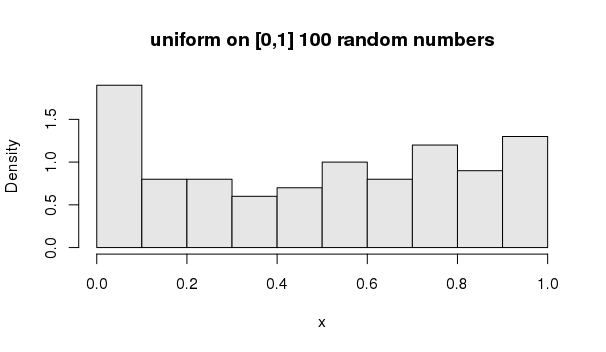
\includegraphics[scale=.4]{chapters/images/hist_100}
\end{figure}

  \begin{lstlisting}[language=R]
  
x=runif(100000)  
hist(x,probability=TRUE,col=gray(.9),main="uniform on [0,1] 100000 random numbers"
# Read  the documentation of hist function to understand the arguments 

\end{lstlisting}

The plot is now looking like the one in fig  hist10000

\begin{figure}
\centering
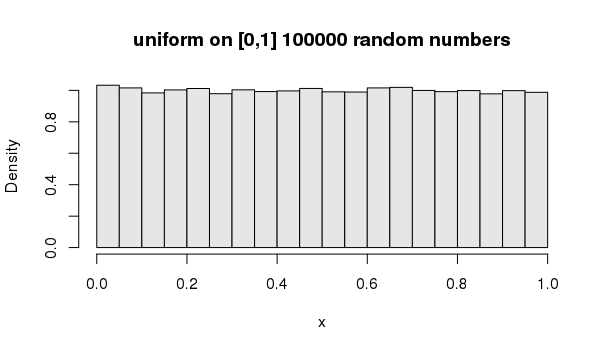
\includegraphics[scale=.4]{chapters/images/hist_10000}
\end{figure}

It may be noted that the plots you get  may look slightly different as we are generating random numbers.
If  you want to plot density function, use dunif to  along with curve function.
 \begin{lstlisting}[language=R]
x=runif(100)  
 curve(dunif(x,0,1))  #  read documentation of curve. 
\end{lstlisting}

   \section{Central limit theorem}
   The  central limit theorem is probably the most important theorem in statistics. let $x_1,x_2\cdots x_n$ be random samples from any distribution with mean $\mu$ and variance $\sigma ^2$ , central limit theorem states that  for large sample size n the sampling distribution of sample mean $\hat{x} = \frac{1}{n}\sum{i=1}^{n} X_i$ is approximately normal with mean $\sigma$ and variance $\sigma^2 / n$ 
   \section{Central limit theorem in R}
   The binomial distribution with parameters n and p is the discrete probability distribution of the number of successes in a sequence of n independent yes/no experiments, each of which yields success with probability p.
    Consider a binomial distribution with N=20 p=0.25. We do 25 trial. Each trial has a probability of success 0.25.
    We can generate random numbers distributed using this binomial distribution using 
    rbinom(1,n.p). This function returns the number of successes  in n trials.
    The first parameter is the number of random numbers to be generated. eg. rbinom(10,n,p) will generate 10 such random numbers. 
    The mean of binomial distribution is np and the variance is np(1-p). 
    
    Let us draw 10 samples from the above distribution and find out the average.  We demote it as one experiment.
    
     
\begin{lstlisting}[language=R]
 n=25
 p=0.25;
 
 X=rbinom(10,n,p)
\end{lstlisting}
 Let us compute the average of these samples
 \begin{lstlisting}[language=R]
 Y=sum(X)/10
\end{lstlisting}

The average of the distribution is 6.25 (np). Compare it Y. It will be some where near 6.25.
Now let us do the above operation 10 times and compute average in each  case. Here we are sampling 10 numbers from a binomial distribution 10 times and finding out how the averages behave.  We are doing 10 experiments.


 \begin{lstlisting}[language=R]
 Y=matrix( rbinom(100,n,p ), 10, 10) ) # Y is a 10 by 10 matrix. Each row contains 10 numbers sampled from the binomial distribution.
 Y  # Examine Y

 Z= rowSums(Y) /10  # Z contains 10 averages  

 hist(Z)    # Find out how  Z is distributed.
 
\end{lstlisting}

The  central limit theorem says that the histogram  of the above averages will approach normal distribution as we do more and more experiments.
 Let us do 100 such experiments.
 
 
 \begin{lstlisting}[language=R]
 Y=matrix( rbinom(1000,n,p ), 100, 10) ) # Y is a 100 by 10 matrix. Each row contains 10 numbers sampled from the binomial distribution.
 Y  # Examine Y

 Z= rowSums(Y) /10  # Z contains 100 averages  

 hist(Z)    # Find out how  Z is distributed.
 
\end{lstlisting}
 
 Repeat it for  1000 experiments 
 
 
 \begin{lstlisting}[language=R]
 Y=matrix( rbinom(10000,n,p ), 1000, 10) ) # Y is a 1000 by 10 matrix. Each row contains 10 numbers sampled from the binomial distribution.
 Y  # Examine Y

 Z= rowSums(Y) /10  # Z contains 1000 averages  

 hist(Z)    # Find out how  Z is distributed.
 
\end{lstlisting}

You can see that the histogram approaches normal
% Correct it with variance.  
\end{document}


